\documentclass[12pt,a4paper]{article}
\usepackage[utf8]{inputenc}
\usepackage{amsmath}
\usepackage{amsfonts}
\usepackage{amssymb}
\usepackage{graphicx}
\usepackage[T1]{fontenc}
\usepackage{imakeidx}
\begin{document}
\begin{center}
\textbf{UNIVERSIDAD MARISTA}
\begin{figure}[htb]
	\centering
	
\includegraphics[scale=1.1]{logo_marista_trabajo_titulacion.jpg}
\end{figure}\\
RECONOCIMIENTO DE  VALIDEZ OFICIAL  DE ESTUDIOS\\
 $No. 992135$ DE FECHA 25-II-99, OTORGADO \\
POR LA SECRETARÍA DE EDUCACIÓN PÚBLICA \\
\textbf{Desarollo de una Aplicación que Proporcione Portafolios de Inversion  por medio  del Modelo de Markowitz y Cadenas de Markov}\\

\textbf{Tesís}\\
QUE PARA OBTENER EL TITULO DE : \textbf{Actuario}\\
P R E S E N T A\\
Arredondo Pérez Leonardo\\
CIUDAD DE MEXICO 2022\\
\end{center}
\newpage
	\tableofcontents
	\newpage
		\section{Introducción}
		\section{Problematica}
		A lo largo de la historia las personas han tenido la necesidad de realizar intercambios de bienes y servicios, cuando las necesidades de estas transacciones fueron evolucionando  las personas tuvieron la necesidad de crear un sistema financiero, para que estas estén protegidas y reguladas, como  define (BANXICO, s.f.) el sistema financiero es:\\ 
\hspace{5mm}"El conjunto de instituciones, mercados e instrumentos en el que se organiza la actividad financiera, para movilizar el ahorro a sus usos más eficientes”.\\
En la figura 1 exponemos, la estructura del sistema financiero mexicano.\\
\begin{figure}[htb]
	\centering
	\caption{Estructura del Sitema Financiero Mexicano}{{\footnotesize Fuente: Elaboración propia-Igleses, s.f.}}
	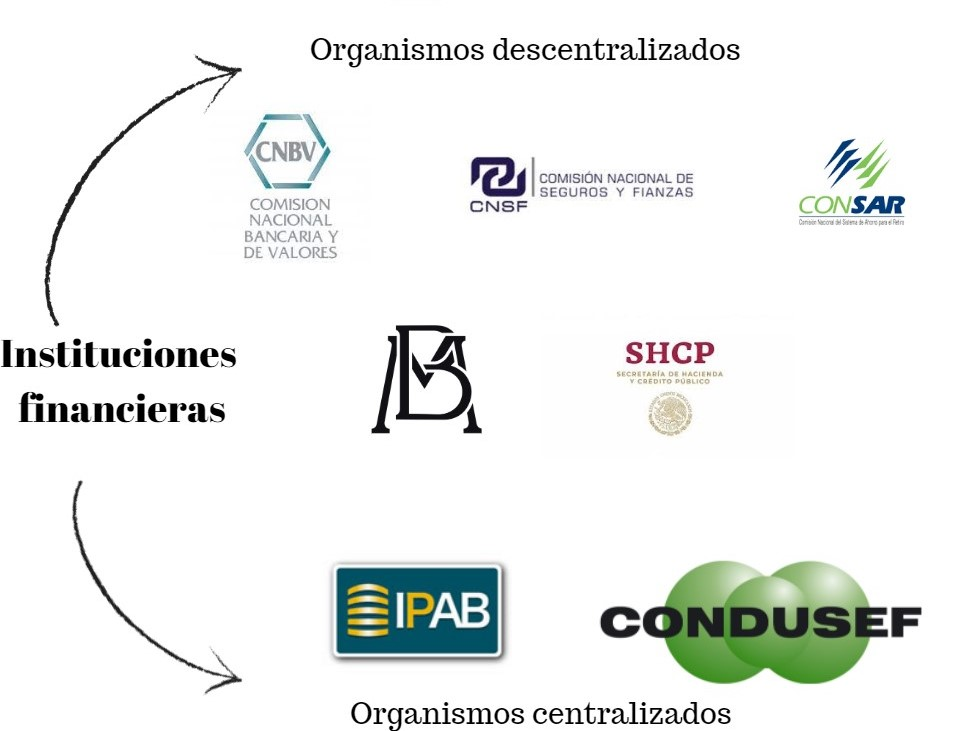
\includegraphics[scale=0.4]{estructurasfm.jpg}
\end{figure}\\
Un mercado finanicero, es todo lugar fisico o digital en donde se compran o venden activos financieros\\
Dentro de este sistema financiero tenemos cinco mercados, los cuales son:
\begin{enumerate}
\item Monetario
\item Capitales
\item Materias primas
\item Divisas
\item Derivados
\end{enumerate}
Para nuestra investigación nos enfocaremos en el mercado de capitales, de acuerdo con (Peiro,2015), este se define como:\\
"El mercado de capitales es aquel al que acuden los agentes del mercado tanto para financiarse a medio y largo plazo (superior a 18 meses) como para realizar inversiones. Al negociarse activos a más largo plazo que en el mercado monetario, incorpora un mayor riesgo."\\
%%Las principales caracteristicas de este mercado son:\\
		\section{Justificación}
		%%Sobre los modelos
		Como mencionan   Chen, J. y Kawaguchi, Y(2018)\\
   "Aunque el modelo de media-varianza, CAPM y el modelo multifactorial son lógicamente simples y útiles en la práctica, son modelos lineales estáticos de un solo período, que difícilmente pueden ajustarse al mundo real"
		%%para que esta aplicación
		\section{Formulación del problema}	
		¿Con qué nivel de confianza podemos asegurar que los portafolios generados nos den un retorno de la inversión mayor al $100\%$?
		\section{Objetivos}
			\subsection{General}
			Desarollar una apliación, que proporcione portafolios de inversión, con el uso del modelo de Fama adn French y cadenas de Markov, que nos otorguen un retorno sobre la  inversion mayor a $100\%$.
			\subsection{Especificos}
			\begin{itemize}
			\item Calcular el portafolios que reflejen el comportamiento del mercado de acuerdo al modelo Fama and French. 
			\item Modelar el comportamiento del mercado a la alza o  a la baja con cadenas de Markov.
			\item Modelar los precios de las empresas con ecuaciones diferenciales estocasticas.
			\item Proporcionar los  portafolios a invertir.
			\end{itemize}
		\section{Hipótesis}
		\section{Marco Teórico}
		\section{Capítulo 1: Aplicaciónes Web}
		\section{Capítulo 2: Modelo Fama and French}
		\section{Capitulo 3: Cadenas de Markov}	
		\section{Metodologia}
		\section{Resultados}
		\section{Concluciones}
		\section{Bibliografía}
		\begin{enumerate}
		\item Alfonso Peiro Ucha, 17 de diciembre, 2015 Mercado de capitales. Economipedia.com
		\item Chen, J., y Kawaguchi, Y. (2018). Multi-factor asset-pricing models under markov regime switches: Evidence from the chinese stock market. International Journal of Financial Studies, 6(2), 54.
		\end{enumerate}				
\end{document}